
\documentclass[12pt,bibliography=totoc]{article}

\usepackage{graphicx}
\usepackage{times}
\usepackage{changepage}
\usepackage{textgreek}
\usepackage{amsmath}
\usepackage[left=2.5cm, right=2.5cm, top=2.5cm, bottom=2.5cm]{geometry}
\usepackage{amsmath}
\usepackage{booktabs}
\usepackage{array}
\usepackage{float}
\usepackage{natbib}
\usepackage{fancyhdr}
\graphicspath{ {./images/} }
\usepackage{placeins}
\usepackage{graphicx}
\usepackage{subcaption}
\usepackage{setspace}
\singlespacing
\usepackage{booktabs,amsfonts,dcolumn}
\newcolumntype{d}[1]{D..{#1}}
\newcommand\mc[1]{\multicolumn{1}{c}{#1}} % handy shortcut macro
\usepackage[justification=centering]{caption}
\usepackage[colorlinks=true,allcolors=blue]{hyperref}%
\usepackage{graphicx}
\usepackage{tabularx}
\usepackage{tikz}
\usepackage[toc, page]{appendix}
\usepackage[nottoc]{tocbibind}
\usepackage{indentfirst}


\pagestyle{fancy}
% Clear the header and footer
\fancyhead{}
\fancyfoot{}
% Set the right side of the footer to be the page number
\fancyfoot[R]{\thepage}



\begin{document}


\begin{titlepage}
  % \vspace*{\stretch{1.0}}
  % \begin{center}
   %   \Large\textbf{Országok és vállalatok multi-dimenziós összekötöttségének vizsgálata, különböző pénzügyi instrumentumok mentén}\\
    %   \bigskip
    %  \large\textit{Kotró Balázs}\\
    %  \medskip
    %  \large{Komplex vizsga - Kutatási tanulmány}
   %\end{center}
  % \vspace*{\stretch{2.0}}
%\end{titlepage}




 \begin{center}
\Huge\textbf{Interconnectedness - Working title}\\
 
\vspace{3cm}


 \Large\textit{Milan Badics - Balazs Kotro}
 
 \vspace{4cm}
Par gondolat a formazasrol: 12-es betumeret, times new roman, 1-es sorkoz, tehat eleg suru, ennel elkepzelheto, hogy hosszabb lesz, ha ezeket a megkoteseket elengedjuk. Minden egyes fejezetet most kulon oldalon kezdek igy jobban latjuk, hogy mennyit fog kitenni.  \textcolor{red}{pirossal} a te megjegyzeseid vannak jelolve.

Az elbeszeles ideje meg nem tisztazott, hogy mult vagy jelen ido lenne a jobb
\vspace{4cm}
\end{center}

\begin{abstract}
Ezt megirjuk kesobb
\end{abstract}


\end{titlepage}

\newpage

\section{Introduction and literature review}


The subprime crisis renewed the interest in analyzing the co-movement of different financial instruments and systemic risk related studies came to the forefront. Shocks can be transmitted differently across various assets, therefore it is convenient to achieve awareness both for regulators and other market participanst in order to react more efficiently. Understanding such network structures are valuable for reducing potential damage and making appropriate future decisions. Analysis of the interconnectedness of different assets plays crucial role in systematic risk assessment. Furthermore, during crises the strength of connections sharply increases and risk spills over across financial institutes and sovereign bonds, as it happened during the Financial Crisis of 2007-2009 and during the European Sovereign Crisis (\cite{diebold2012better}). \textcolor{red}{IDE KELL MAJD HIVATKOZÁST KERESNI}

Because the financial system is a huge complex interactive system, in recent years scholars began using complex network theory to investigate the interconnectedness of financial institutions. \cite{acemoglu2015systemic} pointed out that in smaller financial systems, shocks make the densely interconnected network steadier, however after a certain size the opposite applies. According to \cite{elliott2014financial}, diversification initially allows failure cascades to travel within the system, but as it increases further, organizations are better insured against one another's failures. Depending more on other participants makes personal sensitivity lower on own investments. \textcolor{red}{SZERINTEM ITT VAN MÉG 1-2 FONTOS CIKK RÁNÉZEK MAJD}

In the empirical literature there are several methods to measure connectedness. In the last decade the widespread methods are Granger causality network (\cite{billio2012econometric}), CoVaR (\cite{adrian2008federal}), MES (\cite{acharya2012capital}) and numerous studies appeared based on the Vector AutoRegressive Diebold-Yilmaz (DY) framework (\cite{diebold2009measuring}, \cite{diebold2012better}). Compared to CoVaR and MES methods the advantage of Granger causality based frameworks is the ability to examine the network both micro (pairwise connectedness) and macro (total connectedness) level. As a result, these methods have been often used to analyse the network on different asset classes like equities, bonds, exchange rates or commodity prices. Most analysis focus on the whole system or some subpart.The dynamics of individual assets' role in the system have not been explored yet. \textcolor{red}{IDE KELL hivatkozások összeszednem}

\smallskip{}
\textcolor{red}{KELLENE EGY KOINTEGRÁCIÓT Nem szokta vizsgálni bekezdés}
\smallskip{}

Central banks traditionally rely on the co-movement of different maturities of yield curves to make effective monetary policy decisions. According to the expectations hypothesis, long-term interest rates are influenced by current and expected future short-term interest rates. However, increasing globalization of financial systems and structural changes across economies have disrupted the integration of the maturity spectrum of different yield curves. Short-end movements are more exposed to monetary policy decisions, so their interconnectedness is more consistent with the alternation of business cycles. The long end of the yield curve is mainly affected by global investment, with current preferences and risk appetite being the primary drivers. The integration of distant maturity points is driven by global capital flows and the volume of investments. \textcolor{red}{IDE MINDENKÉPP KELLENEK HIVATKOZÁSOK}

Usually, a tenor structure consists of multiple maturities which means one-one individual time series. It is challenging to deal with such a magnitude of data, therefore in raw format the yield curve itself is not used. \cite{fernandez2016using} examined only the 10Y yield curve point on EMU countries while \cite{claeys2014measuring} chose the spread between EU government bond yieldsand German sovereign bondyield, also considering 10 years of maturity. \cite{ahmad2018financial} picked bond indices to analyze and \cite{sowmya2016linkages}
decomposed the yield curve to Level, Slope and Curvature factors with the Diebold-Li dimension reduction technique. Multilayer networks, in which the links in each layer represent different types of connections between the same nodes, can combine different measures of interconnectedness to effectively describe complex financial systems. Such networks are already widely used in dependency networks of financial markets. However, few literatures consider multilayer networks to study the interconnectedness of the financial system from the perspective of information propagation. \textcolor{red}{EZT KI KELL BŐVÍTENEM}

We are eager to find the less and most interconnected participants of our system via understanding the connections not only between particular factors, but involving all three of them. We are also curious for the behavior of such linkages during time, thus besides static analysis we performed rolling window-based tests as well. Our contribution to the existing literature is fourfold. We analyze the interconnectedness of different yield curve factors with the consideration of cointegration among the time series. This is the first study which examines the crosswise causality connections among Level, Slope and Curvature. We chose developed economies from all over the World in order to achieve a wide geographical coverage. \textcolor{red}{ITT LEHET KELLENE MÉG MAGYARÁZAT}

We find, that there is cointegration between the yield curve factors, therefore our modelling approach (Toda-Yamamoto method) is justified. There is a not negligible amount of significant cross connections among these factors. The Level drives the highest number of linkages while the Curvature is the main receiver. Slope is ranked as second in both comparisons. USD factors have the most net connections (outgoing –incoming) thus it can be considered as the driver of the system. Our dynamic approach shows that during a recession period the sum of the connections in the network increases which statement is supported with different window sized robustness checks.


\bigskip{}
Itt volna meg nehany hivatkozas otletem, itt hagyom magyarul a szoveget ahogy megirtam:
\bigskip{}


\textcolor{cyan}{\cite{yang2016interdependence} az európai kötvények függetlenségét vizsgálják meg és azt találják, hogy a hozamgörbe hosszú vége sokkal integráltabb a rövid lejáratoknál. A hosszú lejárat a befektetői preferenciák szerint, míg a rövid a gazdasági ciklusoktól függ. Összevetve a lejárati szerkezetet, az összekapcsoltság diverz mintát mutat.
\cite{engsted2007comovement} a német és amerikai kötvénypiac együttmozgását tanulmányozzák és jelentős okságot tapasztalnak az amerikai kötvények felől a németek irányába és csak gyenge kapcsolatot fordítva.
\cite{davies2007international} az angol, német, japán és svájci államkötvényindexek integrációját vizsgálja és mind a négy ország piacain azonos trendeket figyel meg.
\cite{vo2009international} ázsiai kötvényeket vet össze fejlett országok (USA és Ausztrália) állampaírjaival. Arra az eredményre jut, hogy az ázsiai oszágok és az Egyesült Államok közötti, ilyen értelemben vett integrációja alacsony szintű.
Bizonyos tanulmányok a kötvények közötti volatilitás átterjedést vizsgálják. 
\cite{ahmad2018financial} kutatásának középpontjába a BRICS államok, valamint három globális kötvénypiaci index (USA, Európai Monetáris Unió, Japán) került és hozam, illetve volatilitásterjedési vizsgálatot végeznek rajtuk. Azt tapasztalják, hogy a redszerbe elsődlegesen Oroszroszág, majd Dél-Afrika által jutnak be a sokkok. Kína és India kevésbé kitett, így ezek az országok fedezési célokat szolgálhatnak.
\cite{fernandez2016using} az EMU tagállamait tanulmányozva arra jutnak, hogy nyugodt időszakban a volatilitás a mag államokból a periféria felé terjed, de az európai szuverén válság idején ez az irány megfordul.
Más cikkek a kötvények hozamfeláraiból indultak ki. 
\cite{antonakakis2013sovereign} az eurozóna tagállamainainak kötvényfelárait vizsgálják és azt tapasztalják, hogy a variancia 61\%-át a más országokból való átgyűrűzés magyarázza. 
\cite{claeys2014measuring} is Európai Uniós országok kötvényfelárait vizsgálják (16, nem csak eurozóna országok) és konklúziójuk szerint az összekötöttség nagy mértékben nőtt a 2008-as pénzügyi válság óta.
Néhány szerző az adott ország hozamgörbéjére ható globális faktorokat elemzi. \cite{driessen2003common} főkomponenselemzéssel találják meg a kötvényhozamokat mozgató faktorokat és szignifikáns pozitív kapcsolatot állapítanak meg a hozamgörbe szintjei között a vizsgált országok esetén.
\cite{abbritti2013global} könyvükben affin lejárati szerkezetű hozamgörbékre ható globális faktorokat elemeznek és arra a következtetésre jutnak, hogy ezek a görbe hosszú végét befolyásolják.
\cite{diebold2008global} létrehozzák dinamikus hozamgörbe modelljüket és kimutatják a Szint, Meredekség és Görbület faktorok szignifikanciáját.
Ezt \cite{bae2011global} kiegészítik regionáls attribútumokkal is ázsiai országok alapján, de a globális együtthatókat erősebbnek találják a lokálisoknál.
\cite{sowmya2016linkages} négy fejlett nyugati, és hét ázsiai ország hozamgörbéinek teljes lejárati stuktúráját modellezik. A Diebold-Li faktorok közötti varaiancia terjedését vizsgálva azt kapják, hogy a Szint faktorok között a legnagyobb az átterjedés, ezt követi a Meredekség, majd a Görbület.}




\newpage 


\section{Methodology}
\noindent
\subsection{The Nelson-Siegel yield curve model and the Diebold-Li decomposition}


%A hozamgörbe modelleknek az a célja, hogy lehetővé tegyék a hozamgörbe illesztését, ezt követő paraméteres struktúrán alapuló interpolációját és extrapolációját, amely megegyezik más, nem parametrikus (statisztikai alapú) illesztési modellekkel, például a simító spline-okkal.
The target of the yield curve models is to enable the fitting of the yield curve, then the parametric interpolation and extrapolation afterwards, which is in line with the non-parametric (statistics based) fitting methods, such as smoothing splines.
%A statisztikai modellek mellett \cite{diebold2006forecasting} modellje terjedt el a tudományos irodalomban és az ipari alkalmazásban egyaránt. A módszer a \cite{nelson1987parsimonious} által kidolgozott hozamgörbe modellezés dinamikus kiegészítése. A piacon megfigyelt hozamgörbe a  következő egyenletnek feleltethető meg:
Besides the statistical approaches, the model of \cite{diebold2006forecasting} spread widely both in the academic literature and in industrial applications. This method is the dinamic extension of the yield curve modelling elaborated by \cite{nelson1987parsimonious}. The observed yield curve can be described with the following equation:

%---------------------------------------------------------------EQ1------------------------------------------------------------------------------------------------------------
\begin{equation}
y_{\tau}=\beta_{1}+\beta_{2}\left ( \frac{1-e^{-\lambda\tau}}{\lambda\tau} \right )+\beta_{3}\left ( \frac{1-e^{-\lambda\tau}}{\lambda\tau} -e^{-\lambda\tau}\right )
\end{equation}
%-------------------------------------------------------------------------------------------------------------------------------------------------------------------------------

%where \textit{y\textsubscript{it}(m\textsubscript{it})} are the observed rates on a given date \textit{i} and maturity \textit{t}, and \textbeta\textsubscript{1t}, \textbeta\textsubscript{2t}, \textbeta\textsubscript{3t} 

where $y_{\tau}$ are the realized values for $\tau$ maturity, $\beta_{1}$, $\beta_{2}$ és $\beta_{3}$ are time varying parameters, and $\lambda$ is the exponential decay factor.
The Nelson-Siegel model is a simple way of yield curve fitting, while the approach is capable to capture the stylized facts observable in the market, such as the usual shape of yield curves (forward sloping, inverse, humped).
% miközben az eljárás képes megragadni a piacon megfigyelhető stilizált tényeket, például a görbe megszokott alakjait (emelkedő, inverz, púpos). 
The $\beta_{i}$ parameters have an economic meaning, $\beta_{1}$ represents the long end of the yield curve,  $\beta_{2}$ is the short term component, while $\beta_{3}$ mimics the middle interval. According to the interpretation of \cite{litterman1991common} these factors can be considered as the Level, Slope and Curveture of the yield curve, accordingly. These components can be utilized for interest-rate asset immunization as well. Besides simple estimation, the model of \cite{diebold2006forecasting} has two further advantages compared to non-parametric approaches. First is, that the extrapolation is more accuratge thanks to the model being exponential. The other is the upper mentioned Litterman interpretation with which understanding and comapring results being much easier.
 
With the extension of \cite{diebold2006forecasting} the Nelson-Siegel model becomes dynamic (the curve fits on multiple observations), which is achieved  the below three steps:

\begin{itemize}
%\item A Nelson-Siegel modelt a legkisebb négyzetek elve alapján illesztik (Ordinary Least Squares - OLS)  minden megfigyelési időpontra, megbecsülve ezáltal a $\beta_{1}$ ,  $\beta_{2}$ ,  $\beta_{3}$  paramétereket. (A $\lambda$ paraméter rögzítésre kerül, így az eljárás lineáris.)
\item The Nelson-Siegel model is fitted based on the Ordinary Least Squares principle, estimating the $\beta_{1}$ ,  $\beta_{2}$ ,  $\beta_{3}$  parameters. (The $\lambda$ parameter is being fixed, therefore the approach is linear.)
%\item A rendszer dinamikáját egy vektor-autoregresszív (VAR) modell jellemzi, az első szakaszban becsült  $\beta_{1}$,  $\beta_{2}$ és $\beta_{3}$ paraméterek alapján. 
\item The dyniamics of the system are described by a Vector AutoRegressive (VAR) model, based on the $\beta_{1}$,  $\beta_{2}$ és $\beta_{3}$ parameters estimated in the first phase.
%\item A $\beta$ paraméterek előrejelezhetőek a VAR modellel és (1) egyenletbe való visszahelyettesítésük-kel a jövőbeli hozamgörbe megbecsülhető.
\item The $\beta$ parameters can be predicted with the VAR modellel and replacing them to  equation (1) the future yield curve is predictable.

\end{itemize}

Additional stylized facts achieved by the Diebold-Li model is the high persistance of time dynamics (same yield curve tenors are highly dependent on past values) and the fact that the long end of the curve is less volatile than the short end.


\subsubsection{The Toda-Yamamoto model}

The \cite{toda1995statistical} method uses the followig premise: the classic Granger causality test (\cite{granger1969investigating}) obtained by a VAR model, may cause a non-stationarity problem, since it does not account the potential cointegration between the used time series.
%A VAR modellel kapott klasszikus Granger oksági teszt (\cite{granger1969investigating}) használatakor nemstacionaritási probléma léphet fel, mivel az nem számol az idősorok között fellépő potenciális kointegrációval. 
\cite{toda1995statistical} point out, that the usual Wald test leads to integrated or cointegrated VAR model, which eventually results spurious Granger causal connections. The Toda-Yamamoto approach eliminates this shortcoming by introducing a modified Wald test (MWald) which has restrictions on the parameters of the VAR$(p)$ model. The test is based on a  $\chi_{p}$  distribuiton, where $p' = p + d^{max}$. The order of VAR is increased artificially, $p$ gets increased by $d^{max}$ which is the maximal order of the integration. Then a VAR with order of $(p + d^{max})$ is estimated, where the last  $d^{max}$ lag coefficient is ignored. A VAR$(p + d^{max})$  model is desribed by equations a (2) and (3):

%---------------------------------------------------------------EQ2------------------------------------------------------------------------------------------------------------
\begin{equation}
Y_t=\alpha_0+\sum_{i=1}^{p} \delta_{1i} Y_{t-i}+\sum_{j=p+1}^{d^{max}} \alpha_{1j} Y_{t-j}+\sum_{j=1}^{p} \theta_{1j} X_{t-j} +\sum_{j=p+1}^{d^{max}} \beta_{1j} X_{t-j}+\omega_{1t} \
\end{equation}


%---------------------------------------------------------------EQ3------------------------------------------------------------------------------------------------------------
\begin{equation}
X_t=\alpha_1+\sum_{i=1}^{p} \delta_{2i} Y_{t-i}+\sum_{j=p+1}^{d^{max}} \alpha_{2j} Y_{t-j}+\sum_{j=1}^{p} \theta_{2j} X_{t-j} +\sum_{j=p+1}^{d^{max}} \beta_{2j} X_{t-j}+\omega_{2t} \
\end{equation}
%-------------------------------------------------------------------------------------------------------------------------------------------------------------------------------

where $\alpha, \delta, \theta$ and $\beta$ are model parameters, $p$ is the optimal lag of the original VAR model, $\omega_{1t}$ és $\omega_{2t}$  are the errors of the VAR model, and $d^{max}$ is the maximal order of integration in terms of the Toda-Yamamoto model.
hereby based on (2), there is a Granger causality between $X$ and $Y$, $\delta_{1i}  \neq 0$ for all $i$. In the same manner, based on (3),  Granger causality is observable between $Y$ and $X$, if  $\delta_{2i}  \neq 0$ for all $i$.
From the VAR$(p+d^{max})$  model, the Toda–Yamamoto approach is realized in three steps: 

\begin{itemize}
\item Perform $d^{max}$  ordered stationarity test on all time series with applying ADF (Augmented Dickey-Fuller test), KPSS (Kwiatkowski-Phillips-Schmidt-Shin test) and PPE ( Phillips-Perron test) tests individually or in combination. 

\item Determine the optimal lag, $(p)$ with the maximal consistency of the AIC (Akaike's Information criterion), the FPE (Akaike's Final Prediction Error), the BIC (Bayesian Information Criterion), the HQ (Hannan-Quinn criterion) and the LR (Lielihood Ratio test) criteria.

\item With the application of the upper mentioned parameters, rejecting the Granger test between $X$ and $Y$ means a causality relation in Toda-Yamamoto terms. Bivariate rejection suggests a mutual causal relationship between the variables.
\end{itemize}




\newpage 



\section{Data}

The yield curve time series of the countries were downloaded from Bloomberg. Twelve developed countries were involved into the examination universe, which cover more geographic regions, since they were selected from different continents. Evenually four regions were defined with three-three suvereigns in each. These are the \textit{Pacific} (Australia, China, Japan), \textit{American} (Canada, Mexico, United States), \textit{Euro-zone} (France, Germany, Italy) and the \textit{Non Euro-zone} (United Kingdom, Norway, Switzerland). Ongoingly they are referred as the three letter abbreviation introduced by Worldbank. Respectively:  AUS, CHN, JPN, CAN, MEX, USA, FRA, DEU, ITA, GBR, NOR, CHE. During the empirical analysis, the yield curve is examined by its whole tenor structure with fifteen different maturities: 3, 6, 12, 24, 36, 48, 60, 72, 84, 96, 120, 180, 240 and 360. These apply for all countries. The firs observation day is 7/1/2004 while the last one is 12/31/2019. The uniusual period is determined by the Chinese yieldcurve since in this case data is available form July 2014 only. Furthermore the effects of recent COVID19 pandemic is exluded from this study, therefore we chose the last day of 2019 for ending the time horyzone. Altogether 4045 we work with 4045 daily observations. Missing data points are forward filled ffrom the previous day.

The inputs of the country yield curves are always zero-coupn bonds, denominated in the local currency of the sovereing. Debt in local currency represents the different interest rate cicle of the economy and represents the domestic monetary policy better. Furthermore the debt denominated in local currency has better liquidity and credit rating then holding the same in USD  (\cite{sowmya2016linkages}). Table \textcolor{red}{2} in the appendix provides descriptive statistics for the 1, 5, 10 and 30 years tenors of each country yield curves. The Level (L), Slope (S) and Curvature (C) factors are calculated by \cite{diebold2006forecasting}, \cite{diebold2008global}, assuming a dynamic Nelso-Siegel model. Figure 1 shows the normalized time series of the factors.

%---------------------------------------------------------------Fig2------------------------------------------------------------------------------------------------------------

\begin{figure}[H]
\centering
\caption{Normlized factor time series}
\begin{subfigure}{.5\linewidth}
\centering
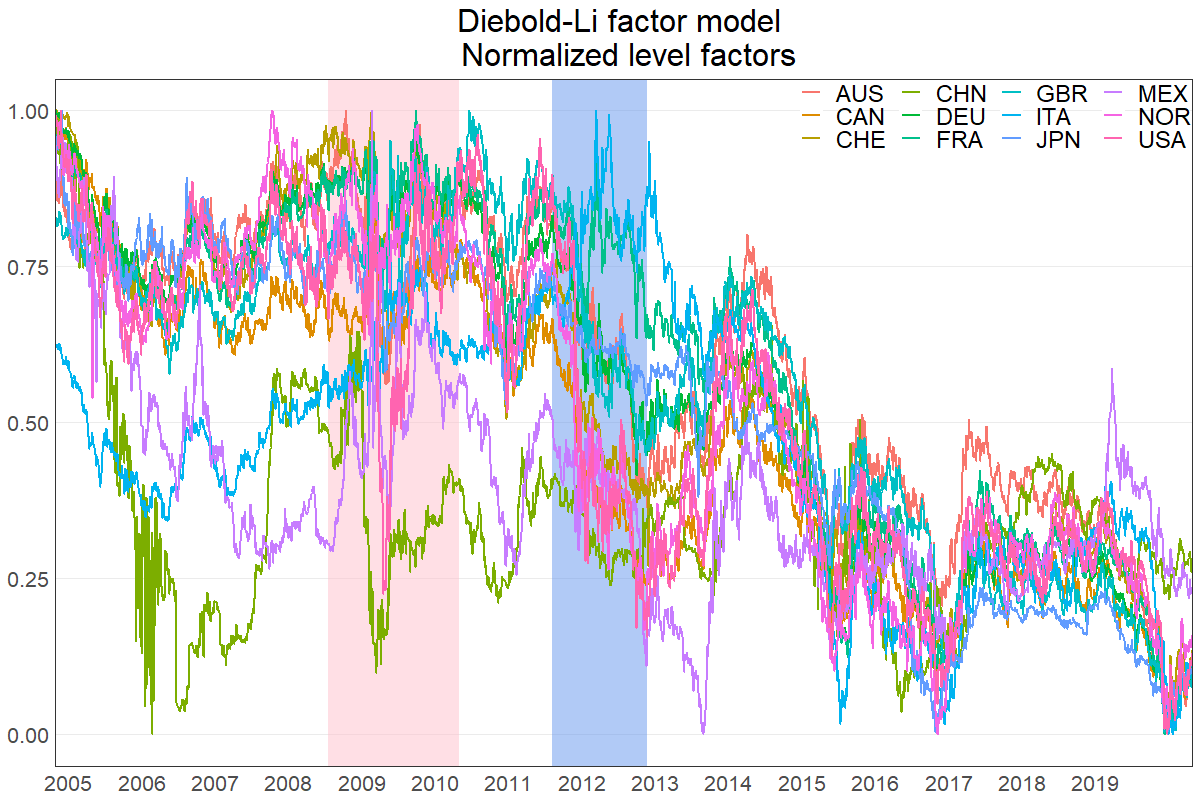
\includegraphics[width=\linewidth]{Normalizedlevel}
\caption{\textbf{Levle}}

\end{subfigure}%
\begin{subfigure}{.5\linewidth}
\centering
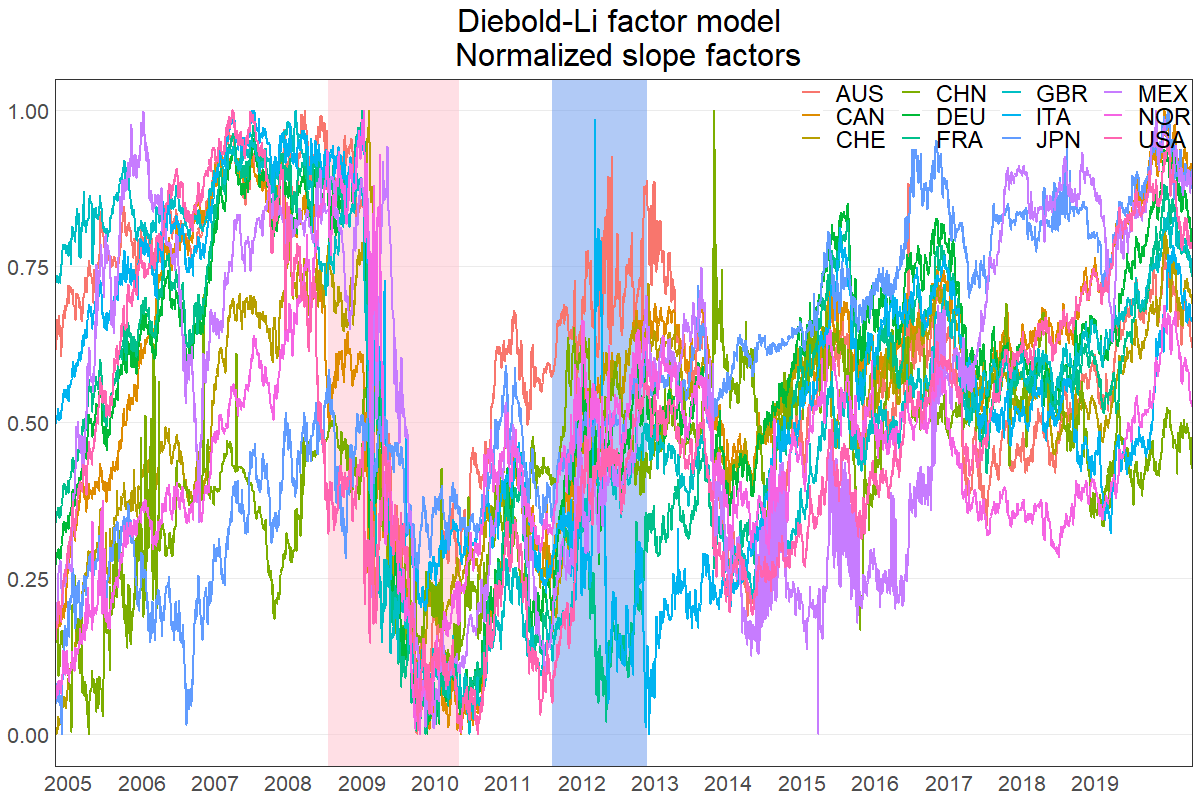
\includegraphics[width=\linewidth]{Normalizedslope}
\caption{\textbf{Slope}}
\end{subfigure}\\[1ex]
\begin{subfigure}{.5\linewidth}
\centering
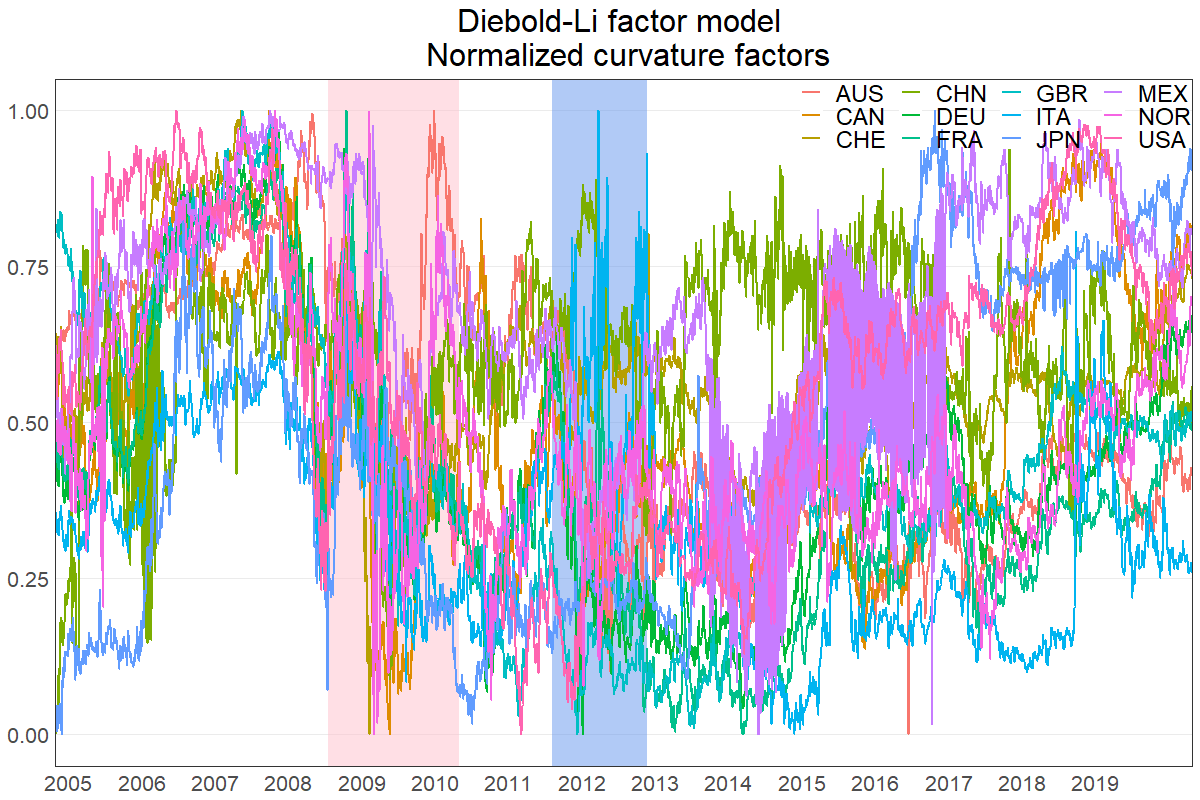
\includegraphics[width=\linewidth]{Normalizedcurvature}
\caption{\textbf{Curvature}}
\end{subfigure}
\end{figure}

%---------------------------------------------------------------------------------------------------------------------------------------------------------------------------

The descriptive statistics of the factors are represented in Table 1. The average Level factor is positive in all cases, highest for Mexico and lowest for Japan. Average Slope refers to the tipical increasing shape of the yield curves (negative values). Slope is negative for all countries meaning that longer maturities have higher values than shorter ones. In absolute terms the USA has the highest Slope, while Australia has the lowest. Potential positive values of Slope represent restricittive monetary politics. Curvature is always negative too, highest for France and lowest for China (in absoluter terms).


%-----------------------------------------------------------------------------------Table1-----------------------------------------------------------------------------
\begin{table}[H]
\caption{Descriptive statistics of yield curve factors}% title of Table
\fontsize{10}{10}\selectfont
\centering % used for centering table
\begin{tabular}{l c c c c c c}% centered columns (4 columns)
\hline\hline   \\ [-1.5ex]               %inserts double horizontal lines
%Case & Method\#1 & Method\#2 & Method\#3 & test \\  [0.5ex]
Factor & Average & Std. dev. & Minimum & Maximum & Jarque-Bera t-stat.  & P value \\ [0.5ex] % inserts table %heading

\hline       \\ [-1.5ex]           % inserts single horizontal line

\textit{Germany}			&		&		&		&		&		&		\\
Level						&	 2.92 &	1.54	&	-0.34	&	5.41	&	347	&	0.00	\\
Slope				&	-1.86	&	1.06	&	-4.54	&	0.14	&	210	&	0.00	\\
\medskip													
Curvature					&	-3.72	&	1.72	&	-7.15	&	0.73	&	234	&	0.00	\\
\textit{Italy}			&		&		&		&		&		&		\\
Level						&	4.78	&	1.29	&	1.98	&	8.00	&	106	&	0.00	\\
Slope				&	-3.43	&	1.57	&	-7.01	&	-0.44	&	183	&	0.00	\\
\medskip													
Görbület					&	-4.25	&	2.24	&	-8.60	&	4.75	&	194	&	0.00	\\
\textit{France}			&		&		&		&		&		&		\\
Level						&	3.39	&	1.37	&	0.26	&	5.48	&	417	&	0.00	\\
Slope				&	-2.24	&	1.19	&	-4.73	&	0.02	&	162	&	0.00	\\
\medskip													
Curvature					&	-4.29	&	1.96	&	-7.82	&	1.07	&	210	&	0.00	\\
\textit{USA}				&		&		&		&		&		&		\\
Level						&	3.96	&	0.99	&	1.88	&	5.87	&	323	&	0.00	\\
Slope				&	-2.41	&	1.55	&	-5.52	&	0.71	&	139	&	0.00	\\
\medskip													
Curvature					&	-3.63	&	2.50	&	-9.58	&	0.72	&	228	&	0.00	\\
\textit{Canada}				&		&		&		&		&		&		\\
Level						&	3.43	&	1.10	&	1.23	&	5.90	&	274	&	0.00	\\
Slope				&	-1.73	&	1.23	&	-4.84	&	0.58	&	251	&	0.00	\\
\medskip													
Curvature					&	-2.49	&	1.63	&	-6.26	&	1.31	&	206	&	0.00	\\
\textit{Mexico}				&		&		&		&		&		&		\\
Level						&	8.58	&	1.28	&	5.56	&	13.41&	834	&	0.00	\\
Slope				&	-2.36	&	1.83	&	-6.14	&	0.67	&	340	&	0.00	\\
\medskip													
Curvature					&	-4.16	&	2.85&	-14.84&	0.49	&	321	&	0.00	\\
\textit{Japan}				&		&		&		&		&		&		\\
Level						&	1.70	&	0.83	&	-0.02	&	3.26	&	406	&	0.00	\\
Slope				&	-1.28	&	0.63	&	-2.83	&	-0.02	&	155	&	0.00	\\
\medskip													
Curvature					&	-3.69	&	1.28	&	-6.03	&	-0.87	&	278	&	0.00	\\
\textit{China}				&		&		&		&		&		&		\\
Level						&	4.02	&	0.62	&	2.70	&	6.52 &	2047	&	0.00	\\
Slope				&	-1.53	&	0.81	&	-3.87	&	1.65 &	275	&	0.00	\\
\medskip													
Curvature					&	-1.24	&	0.92	&	-5.20	&	1.25&	1128	&	0.00	\\
\textit{Australia}			&		&		&		&		&		&		\\
Level						&	4.63	&	1.23	&	1.40	&	6.77	&	262	&	0.00	\\
Slope				&	-0.89	&	0.98	&	-3.87	&	1.00	&	105	&	0.00	\\
\medskip													
Curvature					&	-2.08	&	1.84	&	-6.59	&	2.25	&	296	&	0.00	\\
\textit{Norway}				&		&		&		&		&		&		\\
Level						&	3.22	&	1.12	&	1.02	&	5.23	&	333	&	0.00	\\
Slope				&	-1.22	&	1.07	&	-4.04	&	2.26	&	167	&	0.00	\\
\medskip													
Curvature					&	-1.59	&	1.22	&	-4.68	&	1.73	&	337	&	0.00	\\
\textit{United Kingdom}		&		&		&		&		&		&		\\
Level						&	3.66	&	1.23	&	0.87	&	5.80	&	329	&	0.00	\\
Slope				&	-1.76	&	1.75	&	-5.42	&	1.35	&	211	&	0.00	\\
\medskip													
Curvature					&	-3.33	&	3.02	&	-8.77	&	3.65	&	159	&	0.00	\\
\textit{Switzerland}				&		&		&		&		&		&		\\
Level						&	1.77	&	1.18	&	-0.76	&	3.86	&	289	&	0.00	\\
Slope				&	-1.18	&	0.70	&	-3.32	&	0.91	&	219	&	0.00	\\
Curvature					&	-2.94	&	1.21	&	-7.77	&	0.62	&	543	&	0.00	\\

\hline%inserts single line
\end{tabular}
\label{table:nonlin}% is used to refer this table in the text
\end{table}
%----------------------------------------------------------------------------------------------------------------------------------------------------

%------------------------------------------------ table2---------------------------------------------------------------------------------

\bigskip

\begin{table}
\caption{Results of unit-root tests}
\fontsize{10}{10}\selectfont
\centering% centering table
\captionsetup{justification=centering}

%------------------------------------------------ ADF table----------------------------------------------------------------------------
\begin{subtable}[t]{1\textwidth}
\centering% centering table
\begin{tabular}{l cc cc cc cc cc cc}
\hline\hline \\ [-1.5ex]                         
 

Country	&	\multicolumn{2}{c}{DEU}			&	\multicolumn{2}{c}{ITA}			&	\multicolumn{2}{c}{FRA}			&	\multicolumn{2}{c}{USA}			&	\multicolumn{2}{c}{CAN}			&	\multicolumn{2}{c}{MEX}			\\[0.5ex] 

& value &P 		& value &P 			& value &P  		& value& P         			& value &P				& value &P\\

\hline       \\ [-1.5ex] 

Level	&	-2.30	&	0.45	&	-1.47	&	0.81	&	-2.16	&	0.51	&	-3.66	&	0.03	&	-3.06	&	0.13	&	-3.97	&	0.01	\\
Slope	&	-2.09	&	0.54	&	-2.26	&	0.47	&	-1.64	&	0.73	&	-1.50	&	0.79	&	-1.57	&	0.76	&	-1.88	&	0.63	\\
\medskip
Curvature	&	-2.22	&	0.49	&-3.59	&0.03	&	-2.36	&	0.43	&	-1.62	&	0.74	&	-2.35	&	0.43	&	-2.71	&	0.28	\\

\hline   \\ [-1.5ex]    

Country	&	\multicolumn{2}{c}{JPN}			&	\multicolumn{2}{c}{CHN}			&	\multicolumn{2}{c}{AUS}			&	\multicolumn{2}{c}{NOR}			&	\multicolumn{2}{c}{GBR}			&	\multicolumn{2}{c}{CHE}			\\

 & value &P & value &P& value &P & value &P& value &P & value &P\\

\hline       \\ [-1.5ex] 

Level	&	-2.97	&	0.17	&	-3.69	&	0.02	&	-2.90	&	0.20	&	-2.63	&	0.31	&	-2.16	&	0.51	&	-2.50	&	0.37	\\
Slope	&	-4.85	&	0.01	&	-3.69	&	0.03	&	-2.30	&	0.45	&	-2.72	&	0.27	&	-0.95	&	0.95	&	-3.14	&	0.10	\\
Curvature	&	-2.03	&0.57	&	-5.52	&	0.01	&	-2.61	&	0.32	&	-3.67	&	0.02	&	-1.62	&	0.74	&	-3.14	&	0.10	\\
\hline
\end{tabular}
\caption{\textbf{ADF test results}}
\end{subtable}
\hspace{\fill}
%----------------------------------------------------------------------------------------------------------------------------------------------------
\bigskip 

%------------------------------------------------ KPSS table----------------------------------------------------------------------------
\begin{subtable}[t]{1\textwidth}
\centering% centering table
\begin{tabular}{l cc cc cc cc cc cc}% creating eight columns
\hline\hline \\ [-1.5ex]                         %inserting double-line
%Audio Name&\multicolumn{2}{c}{Sum of Extracted Bits}&\multicolumn{4}{c}{Sum of Extracted Bits} \\ [0.5ex] 

Country	&	\multicolumn{2}{c}{DEU}			&	\multicolumn{2}{c}{ITA}			&	\multicolumn{2}{c}{FRA}			&	\multicolumn{2}{c}{USA}			&	\multicolumn{2}{c}{CAN}			&	\multicolumn{2}{c}{MEX}			\\[0.5ex] 

 & value &P & value &P& value &P & value &P& value &P & value &P\\

\hline       \\ [-1.5ex] 

Level	&	32.89	&	0.01	&	14.58	&	0.01	&	29.87	&	0.00	&	26.85	&	0.01	&	32.18	&	0.01	&	15.24	&	0.01	\\
Slope	&	4.26	&	0.01	&	7.61	&	0.01	&	4.50	&	0.01	&	5.30	&	0.01	&	5.40	&	0.01	&	4.78	&	0.01	\\
\medskip
Curvature	&	8.96	&	0.01	&	10.21	&	0.01	&	15.21	&	0.01	&	7.34	&	0.01	&	4.59	&	0.01	&	4.92	&	0.01	\\


\hline   \\ [-1.5ex]    

Country	&	\multicolumn{2}{c}{JPN}			&	\multicolumn{2}{c}{CHN}			&	\multicolumn{2}{c}{AUS}			&	\multicolumn{2}{c}{NOR}			&	\multicolumn{2}{c}{GBR}			&	\multicolumn{2}{c}{CHE}			\\

 & value &P & value &P& value &P & value &P& value &P & value &P\\

\hline       \\ [-1.5ex] 

Level	&	33.94	&	0.01	&	3.55	&	0.01	&	29.17	&	0.01	&	30.06	&	0.01	&	28.70	&	0.01	&	31.96	&	0.01	\\
Slope	&	33.21	&	0.01	&	14.99	&	0.01	&	7.32	&	0.01	&	1.25	&	0.01	&	7.53	&	0.01	&	5.49	&	0.01	\\
\medskip
Curvature	&	15.95	&	0.01	&	2.91	&	0.01	&	24.67	&	0.01	&	11.56	&	0.01	&	13.33	&	0.01	&	5.67	&	0.01	\\


\hline
\end{tabular}
\caption{\textbf{KPSS test results}}

\end{subtable}
\hspace{\fill}
%----------------------------------------------------------------------------------------------------------------------------------------------------
\bigskip

%------------------------------------------------ ADF(1) table----------------------------------------------------------------------------
\begin{subtable}[t]{1\textwidth}
\centering
\begin{tabular}{l cc cc cc cc cc cc}% creating eight columns
\hline\hline \\ [-1.5ex]                         %inserting double-line
%Audio Name&\multicolumn{2}{c}{Sum of Extracted Bits}&\multicolumn{4}{c}{Sum of Extracted Bits} \\ [0.5ex] 

Country	&	\multicolumn{2}{c}{DEU}			&	\multicolumn{2}{c}{ITA}			&	\multicolumn{2}{c}{FRA}			&	\multicolumn{2}{c}{USA}			&	\multicolumn{2}{c}{CAN}			&	\multicolumn{2}{c}{MEX}			\\[0.5ex] 

 & value &P & value &P& value &P & value &P& value &P & value &P\\

\hline       \\ [-1.5ex] 

Level	&	-17.05	&	0.01	&	-16.01	&	0.01	&	-15.99	&	0.01	&	-15.79	&	0.01	&	-16.35	&	0.01	&	-16.56	&	0.01	\\
Slope	&	-15.90	&	0.01	&	-14.62	&	0.01	&	-14.59	&	0.01	&	-16.55	&	0.01	&	-16.32	&	0.01	&	-15.19	&	0.01	\\
\medskip
Curvature	&-18.52	&	0.01	&	-18.67	&	0.01	&	-17.65	&	0.01	&	-17.45	&	0.01	&	-16.02	&	0.01	&	-18.88	&	0.01	\\


\hline   \\ [-1.5ex]    

Country	&	\multicolumn{2}{c}{JPN}			&	\multicolumn{2}{c}{CHN}			&	\multicolumn{2}{c}{AUS}			&	\multicolumn{2}{c}{NOR}			&	\multicolumn{2}{c}{GBR}			&	\multicolumn{2}{c}{CHE}			\\

 & value &P & value &P& value &P & value &P& value &P & value &P\\

\hline       \\ [-1.5ex] 

Level	&	-16.55	&	0.01	&	-16.99	&	0.01	&	-15.61	&	0.01	&	-16.43	&	0.01	&	-16.48	&	0.01	&	-15.57	&	0.01	\\
Slope	&		&		&	-18.90	&	0.01	&	-17.87	&	0.01	&	-17.61	&	0.01	&	-16.12	&	0.01	&	-14.59	&	0.01	\\
\medskip
Curvature	&	-17.51	&	0.01	&		&		&	-18.06	&	0.01	&	-17.04	&	0.01	&	-16.45	&	0.01	&	-14.27	&	0.01	\\



\hline
\end{tabular}
\caption{\textbf{ADF(1) test results}}
\end{subtable}
\hspace{\fill}
%----------------------------------------------------------------------------------------------------------------------------------------------------
\bigskip 

%------------------------------------------------ KPS (1) table----------------------------------------------------------------------------
\begin{subtable}[t]{1\textwidth}
\centering
\begin{tabular}{l cc cc cc cc cc cc}% creating eight columns
\hline\hline \\ [-1.5ex]                         %inserting double-line
%Audio Name&\multicolumn{2}{c}{Sum of Extracted Bits}&\multicolumn{4}{c}{Sum of Extracted Bits} \\ [0.5ex] 

Slope	&	\multicolumn{2}{c}{DEU}			&	\multicolumn{2}{c}{ITA}			&	\multicolumn{2}{c}{FRA}			&	\multicolumn{2}{c}{USA}			&	\multicolumn{2}{c}{CAN}			&	\multicolumn{2}{c}{MEX}			\\[0.5ex] 

 & value &P & value &P& value &P & value &P& value &P & value &P\\

\hline       \\ [-1.5ex] 

Level	&	0.04	&	0.10	&	0.13	&	0.10	&	0.06	&	0.10	&	0.03	&	0.10	&	0.06	&	0.10	&	0.08	&	0.10	\\
Slope	&	0.08	&	0.10	&	0.07	&	0.10	&	0.12	&	0.10	&	0.16	&	0.10	&	0.17	&	0.10	&	0.09	&	0.10	\\
Curvature	&	0.05	&	0.10	&	0.02	&	0.10	&0.05	&	0.10	&	0.08	&	0.10	&	0.08	&	0.10	&	0.01	&	0.10	\\


\hline   \\ [-1.5ex]    

Slope	&	\multicolumn{2}{c}{JPN}			&	\multicolumn{2}{c}{CHN}			&	\multicolumn{2}{c}{AUS}			&	\multicolumn{2}{c}{NOR}			&	\multicolumn{2}{c}{GBR}			&	\multicolumn{2}{c}{CHE}			\\

 & value &P & value &P& value &P & value &P& value &P & value &P\\

\hline       \\ [-1.5ex] 

Level	&	0.03	&	0.10	&	0.16	&	0.10	&	0.05	&	0.10	&	0.04	&	0.10	&	0.07	&	0.10	&	0.04	&	0.10	\\
Slope	&	0.03	&	0.10	&	0.03	&	0.10	&	0.04	&	0.10	&	0.08	&	0.10	&	0.24	&	0.10	&	0.14	&	0.10	\\
Curvature	&	0.06	&	0.10	&	0.05	&	0.10	&	0.04	&	0.10	&	0.03	&	0.10	&	0.16	&	0.10	&	0.05	&	0.10	\\


\hline
\end{tabular}
\caption{\textbf{KPSS(1) test results}}
\end{subtable}
\hspace{\fill}
%----------------------------------------------------------------------------------------------------------------------------------------------------
%\label{tab:table1}
\end{table}

%----------------------------------------------------------------------------------------------------------------------------------------------------


Factor time sereies are tested with (\cite{bera1981efficient}) test for normality. Neither of them passes the acceptance criteria therefor null-hypothesis for normaility is rejected. Furthermore ADF and KPSS unit-root tests for stationarity is applied. Curvature for China and Slope for Japan is stationary on the usual 95\% confidence level. The tests can be applied for first differenence of the remaining time series. 

Before differentiating, a pairwise  (\cite{engle1987co} test is applied for determining cointegration. Table 3. represents the ratio of the cointegrated time series aggregated by factors. Besides the diagonal, the Slope - Curvature and the Curvature - Slope pairs both show a value more than 70\%. Since the time series are not stationary on the same order and the ratio of cointegrated time series are high, we consider the Toda-Yamamoto approach to be justified for analyzing connections.

%--------------------------------------------------------------------------------Table3 -------------------------------------------------------
\begin{table}[H]
\caption{Blocked Engle-Granger test} %title of the table

\centering% centering table
\begin{tabular}{l | ccc}% creating eight columns
\hline\hline \\ [-1.5ex]                         %inserting double-line

	&	Level 	&	Slope	&	Curvature	\\
\hline \\ [-1.5ex]  
Level	&	75.694\%	&	44.444\%	&	64.583\%	\\
Slope	&	29.167\%	&	74.306\%	&	71.528\%	\\
Curvature	&	29.167\%	&	78.472\%	&	75.000\%	\\

\hline            
\end{tabular}
\label{table:nonlin}% is used to refer this table in the text
\end{table}

%----------------------------------------------------------------------------------------------------------------------------------------------------

\newpage


\bibliographystyle{te}


\bibliography{research}

\begin{appendices}



\begin{table}[H]
\caption{Descriptive statistics of country yield curve nodes}% title of Table
\fontsize{9}{9}\selectfont
\centering % used for centering table
\begin{tabular}{l c c c c c c}% centered columns (4 columns)
\hline\hline   \\ [-1.5ex]               %inserts double horizontal lines
%Case & Method\#1 & Method\#2 & Method\#3 & test \\  [0.5ex]
Node & Average & St. dev & Minimum & Maximum & \textrho(1)  & \textrho(10) \\ [0.5ex] % inserts table %heading

\hline       \\ [-1.5ex]           % inserts single horizontal line
\textit{Germany} 	&		&		&		&		&		&	\\
1 year	&	0.0256	&	1.6275	&	-0.9690	&	4.6900	&	1.0000	&	0.9960	\\
5 years	&	0.0257	&	1.6324	&	-0.9410	&	4.7670	&	0.9990	&	0.9930	\\
10 years	&	0.0243	&	1.5451	&	-0.7220	&	4.6860	&	0.9930	&	0.9640	\\
\medskip													
30 years	&	0.0228	&	1.4482	&	-0.2440	&	5.1950	&	0.9990	&	0.9880	\\
\textit{Italy}	&		&		&		&		&		&		\\
1 year	&	0.0241	&	1.5327	&	-0.4840	&	8.3940	&	0.9980	&	0.9860	\\
5 years	&	0.0239	&	1.5199	&	0.2370	&	7.8950	&	0.9980	&	0.9850	\\
10 years	&	0.0218	&	1.3876	&	0.8750	&	7.4920	&	0.9980	&	0.9860	\\
\medskip													
30 year	&	0.0188	&	1.1971	&	2.0430	&	7.5840	&	0.9980	&	0.9850	\\
\textit{France}	&		&		&		&		&		&		\\
1 year	&	0.0250	&	1.5891	&	-0.8010	&	4.6570	&	1.0000	&	0.9960	\\
5 years	&	0.0247	&	1.5730	&	-0.7730	&	4.9100	&	0.9990	&	0.9930	\\
10 years	&	0.0231	&	1.4670	&	-0.4150	&	4.8510	&	0.9990	&	0.9910	\\
\medskip													
30 years	&	0.0194	&	1.2351	&	0.4190	&	5.1160	&	0.9990	&	0.9860	\\
\textit{USA}	&		&		&		&		&		&		\\
1 year	&	0.0254	&	1.6128	&	0.0540	&	5.3230	&	1.0000	&	0.9980	\\
5 years	&	0.0194	&	1.2315	&	0.5590	&	5.3010	&	0.9990	&	0.9890	\\
10 years	&	0.0163	&	1.0394	&	1.3890	&	5.3880	&	0.9980	&	0.9830	\\
\medskip
30 years	&	0.0151	&	0.9618	&	1.9920	&	5.8390	&	0.9970	&	0.9760	\\
\textit{Canada}	&		&		&		&		&		&		\\
1 year	&	0.0193	&	1.2301	&	0.3000	&	4.8090	&	1.0000	&	0.9950	\\
5 years	&	0.0180	&	1.1463	&	0.4840	&	4.8010	&	0.9990	&	0.9890	\\
10 years	&	0.0173	&	1.0976	&	0.9830	&	5.0760	&	0.9990	&	0.9870	\\
\medskip													
30 years	&	0.0159	&	1.0118	&	1.3060	&	5.6120	&	0.9980	&	0.9850	\\
\textit{Mexico}	&		&		&		&		&		&		\\
1 year	&	0.0318	&	2.0250	&	1.5120	&	10.5700	&	0.9790	&	0.9880	\\
5 years	&	0.0238	&	1.5108	&	3.7860	&	10.8970	&	0.9860	&	0.9810	\\
10 years	&	0.0213	&	1.3524	&	4.6190	&	12.4130	&	0.9920	&	0.9700	\\
\medskip
30 years	&	0.0195	&	1.2384	&	5.8730	&	12.7260	&	0.9930	&	0.9470	\\
\textit{Japan}	&		&		&		&		&		&		\\
1 year	&	0.0043	&	0.2715	&	-0.3710	&	0.8500	&	0.9990	&	0.9920	\\
5 years	&	0.0076	&	0.4852	&	-0.3960	&	1.6310	&	0.9990	&	0.9900	\\
10 years	&	0.0103	&	0.6563	&	-0.2850	&	2.0500	&	0.9990	&	0.9900	\\
\medskip													
30 years	&	0.0120	&	0.7606	&	0.0530	&	3.2950	&	0.9980	&	0.9850	\\
\textit{China}	&		&		&		&		&		&		\\
1 year	&	0.0115	&	0.7296	&	0.9570	&	4.3820	&	0.9920	&	0.9660	\\
5 years	&	0.0093	&	0.5939	&	1.7820	&	4.8740	&	0.9970	&	0.9730	\\
10 years	&	0.0090	&	0.5702	&	2.4810	&	5.5030	&	0.9930	&	0.9640	\\
\medskip													
30 years	&	0.0097	&	0.6149	&	2.4700	&	6.0090	&		&		\\
\textit{Australia}	&		&		&		&		&		&		\\
1 year	&	0.0279	&	1.7749	&	0.6750	&	7.3760	&	0.9990	&	0.9920	\\
5 years	&	0.0264	&	1.6769	&	0.6390	&	6.9600	&	0.9990	&	0.9900	\\
10 years	&	0.0235	&	1.4971	&	0.8850	&	6.8730	&	0.9990	&	0.9880	\\
\medskip													
30 years	&	0.0190	&	1.2069	&	1.5580	&	6.8880	&	0.9980	&	0.9830	\\
\textit{Norway}	&		&		&		&		&		&		\\
1 year	&	0.0222	&	1.4100	&	0.1990	&	6.2430	&	0.9990	&	0.9940	\\
5 years	&	0.0200	&	1.2734	&	0.5450	&	5.3350	&	0.9990	&	0.9910	\\
10 years	&	0.0188	&	1.1935	&	0.8880	&	5.2760	&	0.9990	&	0.9890	\\
\medskip													
30 years	&	0.0175	&	1.1127	&	0.8820	&	5.2730	&	0.9990	&	0.9870	\\
\textit{United Kingdom}	&		&		&		&		&		&		\\
1 year	&	0.0308	&	1.9558	&	0.0240	&	5.8830	&	0.9990	&	0.9950	\\
5 years	&	0.0259	&	1.6444	&	0.1610	&	5.8210	&	0.9990	&	0.9910	\\
10 years	&	0.0223	&	1.4181	&	0.4000	&	5.5430	&	0.9990	&	0.9890	\\
\medskip													
30 years	&	0.0175	&	1.1099	&	0.9390	&	5.0700	&	0.9990	&	0.9870	\\
\textit{Switzerland}	&		&		&		&		&		&		\\
1 year	&	0.0195	&	1.2405	&	-1.1650	&	3.3750	&	1.0000	&	0.9960	\\
5 years	&	0.0187	&	1.1921	&	-1.1960	&	3.2000	&	0.9990	&	0.9930	\\
10 years	&	0.0188	&	1.1976	&	-1.1380	&	3.4550	&	0.9990	&	0.9910	\\
30 years	&	0.0173	&	1.1006	&	-0.6440	&	3.7330	&	0.9980	&	0.9860	\\

\hline%inserts single line
\end{tabular}
\label{table:nonlin}% is used to refer this table in the text
\end{table}
%----------------------------------------------------------------------------------------------------------------------------------------------------


%----------------------------------------------------------------------------------------------------------------------------------------------------

%----------------------------------------------------------------------------------------------------------------------------------------------------

\end{appendices}


\end{document}

